\documentclass[a4paper,9pt]{article}

\usepackage{a4}
\usepackage{amsmath}
\usepackage{amssymb}
\usepackage{colortbl}
\usepackage{color}
\usepackage{xcolor}
%\usepackage{fullpage}
\usepackage{graphicx}
\usepackage{grffile}
%\usepackage{hyperref}
%\usepackage{multirow}
%\usepackage{caption}
%\usepackage{subcaption}
\usepackage{url}
\usepackage{wasysym}
\usepackage{wrapfig}

\usepackage{listings}
\lstdefinestyle{customc}{
  belowcaptionskip=1\baselineskip,
  breaklines=true,
  frame=L,
  xleftmargin=\parindent,
  language=C,
  showstringspaces=false,
  basicstyle=\footnotesize\ttfamily,
  keywordstyle=\bfseries\color{green!40!black},
  commentstyle=\itshape\color{purple!40!black},
  identifierstyle=\color{blue},
  stringstyle=\color{orange},
}

\lstdefinestyle{customasm}{
  belowcaptionskip=1\baselineskip,
  frame=L,
  xleftmargin=\parindent,
  language=[x86masm]Assembler,
  basicstyle=\footnotesize\ttfamily,
  commentstyle=\itshape\color{purple!40!black},
}
\lstset{escapechar=@,style=customc}

\newcommand{\isrc}[1]{\texttt{#1}}
\newcommand{\oaoo}{once and only once}


\title{
TDT4258 Energy Efficient Computer Design\\
Assignment 2 Project Report
}
\author{
  Edvard Kristoffer Karlsen\\
  \texttt{edvardkk@stud.ntnu.no}
}
\date {}

\begin{document}

\maketitle

\begin{abstract}
  In this report we describe our solution to the second assignment of the
  TDT4258 course: designing and implementing an interactive program to
  generate audio output from the STK 1000 using the AP7000's
  Digital-to-analog.  The program is implemented in C, and runs without
  support of an operating system. At the core of the system is a set of audio
  generation and processing modules which together allow multi-track playback
  using several polyphonic synthesizers. Our system includes an offline tool
  that can convert arbitrary MIDI files to a format suitable for playback on
  the board.  In addition to an in-depth description and discussion of our
  solution, we report on the methodological approach we used to attack the
  assignment, describe our testing scheme, and reflect on our process solving
  the assignment.
\end{abstract}

\section{Introduction}

For the second assignment in TDT4258, we are to write a `bare metal' C program
to play different sound effects when different switches on the STK 1000 are
pressed~\cite{compendium}. It is a requirement to use an interrupt handler to
write sample data to the AP7000's DAC, and also to provide at least three
different sound effects. The primary learning objectives of the assignment are
to gain familiarity with C programming, to learn AVR32 Input/Output control
from C, to learn how to use the AP7000 DAC for sound generation, and to learn
interrupt handling in C for the AVR32~\cite{compendium}.

The assignment text does not give very specific requirements for the
capabilities of the sound generation modules; the primary requirement is that
the systems delivered must be able to generate sound effects in some way.
While a basic monophonic square-wave synthesizer is an acceptable solution,
most ambitious students put significant extra effort into implementing more
sophisticated sound generation and processing systems.  For instance, one
impressive solution created this year supports playback of MOD-format files. 
For our system we aimed to implemented effective live synthesis of many tracks
(each, possibly with many voices) in parallel. Our system supports polyphonic
synthesis using square, triangle, and sawtooth waveforms, and includes a mixer
component that can control several synthesizers at the same time. 

The rest of the text is structured as follows: In Section~\ref{sec:method}
we present the approach we used to attack the assignment. Then, in
Section~\ref{sec:implementation} we discuss the design of the system in
depth.\footnote{I am aware that I have split the `Description and Methodology'
header into two, and used slightly different names for some sections. I assume
this is OK.} Further, in Section~\ref{sec:tests} we discuss how we tested the
system, and report on test results. In Section~\ref{sec:eval}
we evaluate the results of the assignment, and in
Section~\ref{sec:conclusion} we conclude.

\section{Method}
\label{sec:method}
As for the first assignment of the course, we used an iterative approach when
attacking this assignment's problems.  Our work proceeded through the
following steps:

\begin{enumerate}
  \footnotesize
  \item Configuring a tool chain for effective cross-compilation of C programs
      for the AVR32.
  \item Experimentation with a minimal C translation of the program from
      Assignment 1.
  \item Development and testing of modules for controlling the STK 1000's LEDs
      and switches.
  \item Experimentation with the AP7000 DAC, writing random data to the sound
      buffers.
  \item Development and initial testing of the synthesis sound system, and
      translation utilities for MIDI files, on our development machine.
  \item Development and testing of a first version of the full system,
      on-board.
  \item Development and initial testing of the music controller module.
  \item Development and integration testing of the final system version,
      incorporating the controller module for multi-track playback.
\end{enumerate}

\subsection{Implementation rules}
An important aspect in effective and safe system development method, is to
have a good set of guidelines for the coding process and rules for the design
and style of the code written.  Early in the development process, we selected
and a relatively strict set of rules for C code. Our guidelines are given
below, with rationales added where appropriate. 
{
\begin{enumerate}
    \item All code shall build without any compiler complaints or notices for
    the option string {\ttfamily -pedantic -Wall -Wextra -Winline -Werror}.
    (Of course, since we use \texttt{-Werror}, no translation unit with a
    warning-provoking construct could ever compile.)

    \item Abstract data types are strongly preferred
    to `open' structures. \textsc{~~rationale:} Using ADTs, it is easier to
    ensure correct allocation and usage of complex data types. Also, internal
    implementation details can be hidden from client code.

    \item Code is indented according to `K\&R style'. \footnote{With a minor
        exception for asterisk-placement in function headers\ldots}

    \item Recursion is forbidden. \textsc{~~rationale:} While not strictly
    `mandatory' in a secure system, forbidding (co-)recursion makes it much
    simpler to reason about memory usage in a memory-constrained
    or safety-critical system. In particular, using some viable
    formalism, stack overflows can be proven impossible.

    \item Dynamic memory allocation is forbidden. \textsc{~~rationale:} 
    Forbidding dynamic memory allocation is also not `mandatory' -- there are
    many places where a \texttt{malloc} call is a reasonable solution.
    However, in a memory-constrained or highly safely-critical system,
    disallowing dynamic memory allocation removes the possibility of many
    memory-related bugs, and allows one to prove stronger properties about the
    soundness of programs.

    \item As far as overly possible, each logical module should be designed
    and implemented to facilitate testing in isolation.

    \item All procedures are designed to fail fast and cleanly when clients do
    not respect their interface, their assumptions are not satisfied, or other
    exceptional circumstances occur.\footnote{With \emph{exception} we mean
    events that are neither on normal, nor `expected' error-handling control
    flow paths.}
    However, a non-exceptional error,
    such as a ABDAC underrun, is an \emph{expectable} error which does not
    necessarily indicate a logical error in the system. Such errors must be
    handled gracefully.\footnote{Of course, if a constant ABDAC flow was a
    hard requirement, it would not be an `acceptable' error condition.
    However, in our system, \emph{some} audio dropout is not a severe
    problem.}

    \item All code should be as readable and clear and possible. 
    Identifiers should be descriptive and correct, and code segments
    should not be overly complex (a maximum of three nested scopes is a good
    rule-of-thumb). We are not proponents of extensively commenting
    everything; if the code can communicate its intent by itself, it is
    virtually always the best option.  For example, a comment over a complex
    conditional, can often be replaced by a sequence of well-named \isrc{bool}
    variables, or a call to a well-named \isrc{bool}-returning procedure, in
    the style advocated by, for example, Robert C.  Martin~\cite{cleancode}.
    Still, some code segments are necessarily complex and intricate (generic
    clock setup on the AP7000, for example), and such segments must
    always be appropriately commented. 
\end{enumerate}
}


\section{System description}
\label{sec:implementation}

In this section we describe our system. We first give a high-level, black box
description of the system, assuming the view of a user. Then, we discuss the
system's hardware setup. Finally, we discuss each of the system's module in
full depth.

\subsection{User interface}
\label{sec:ui}
The system is controlled using six out of the STK 1000's eight primary
switches. Each of switches 4-7 controls one track. The mapping of switches to
melodies is as follows:
\begin{description}
        \footnotesize
    \item[SW7] The beginning of Ramin Djawadi major theme from the Game of
        Thrones series. 
    \item[SW6] The beginning of Prelude 2 from Bach's Well-Tempered Clavier
        collection.
    \item[SW5] A snippet from a `dungeon' song from one of the Zelda
        games.
    \item[SW4] A short `blipp' sound effect, constructed by speeding up and
        transposing the start of a classical piece.\footnote{Although the
        assignment text states that we should play sound effects, my
        impression is that most students program their boards to play
        \emph{music} for the second assignment, since it in many ways poses a
        bigger challenge. However, I have added this `effect' sound to show
        that the system handles small effect sounds perfectly well, and I
        hope that it is clear that configuring the system to play `game sound
        effects' on all four tracks would be a trivial operation.}
\end{description}
Pressing one of these four switches starts its corresponding synthesizer, and
lights its corresponding LED. A playing track can be stopped by pressing its
corresponding switch again. All four tracks can play at the same time.

Switches 1 and 2 are used to control aspects of playback. Pressing and holding
switch 1 before pressing a track switch for a non-playing track, starts the
corresponding synthesizer in looping mode. Looping tracks are indicated with
blinking LEDs. The same gesture can be used with switch 2 to toggle the
synthesis waveform of a track between the square, triangle, and sawtooth
shapes. All synthesizers are initialised to use square waveforms. 

LED 0 is lighted whenever the main module waits for permission to write data
to the DAC. Generally, this diode being lit is a good thing, while a dark or
almost dark LED 0 suggests underruns in the audio stream.

\begin{figure}[!h]
    \centering
    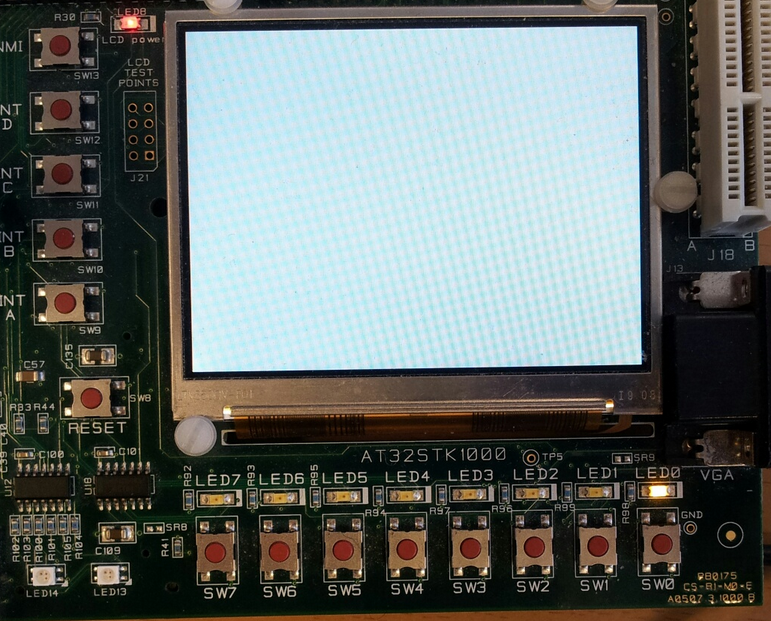
\includegraphics[width=0.4\textwidth]{stk1000_interface.png}
    \caption{The system's hardware interface. No tracks are playing. LED 0 is
    brightly lit, indicating that the systems primarily spends time waiting
    for permission to write to the DAC.}
    \label{fig:interface}
\end{figure}


\subsection{Hardware setup}
\label{sec:hwsetup}
The STK 1000 was configured according to the instructions in the
compendium~\cite[p. 50]{compendium}. As we use both switches and LED diodes,
we connected flat cables between the GPIO connectors and the switches' and
LED's connector as for assignment one. Finally, we connected headphones to the
STK 1000's 3.5 mm audio output, and a JTAG ICE unit to the board's JTAG
connector to enable programming of the AP7000.


\subsection{Modules}
\label{sec:modules}
Our system consists of eight C modules (we do not count the \texttt{utils}
module, which basically consists only of convenience macros). In this section
we describe the interfaces and implementation details of each. The
presentation is given in bottom-up fashion: We first discuss the low-level
modules, before we tie the complete system together in the presentation of the
main module.

\begin{figure}[h!]
    \centering
    \includegraphics[width=0.7\textwidth]{modules.dot.png}
    \caption{System modules (each corresponding to a \texttt{.c/.h}
    pair). Edges indicate module dependencies. Filled grey rectangles indicate
    modules that depend on AVR32 libraries.}
\end{figure}


\subsubsection{LED module}
The LED module is the simplest module in the system.
It provides access to the STK 1000's eight primary LEDs through the following
interface:

\begin{lstlisting}
#define LEDS_CNT          8
#define LED_FROM_LEFT(i)  (LEDS_CNT-1-(i))
#define LED_FROM_RIGHT(i) (i)

void leds_init();
void leds_light(uint32_t led);
void leds_light_all(void);
void leds_turn_off(uint32_t led);
void leds_turn_off_all(void);
void leds_lighted_if(uint32_t led, bool cond);
\end{lstlisting}
Client code is \emph{required} to call \isrc{leds\_init} \oaoo~ to
initialise the module, before calling any other of the module's procedures.
Further, client code is strongly encouraged to use the
\isrc{LED\_FROM\_LEFT} and \isrc{LED\_FROM\_RIGHT} macros in all
calls to the module, even though their current definitions are trivial.

\paragraph{Internals}
This module encapsulates control of the PIOC peripheral port, which is
connected to the STK 1000's eight primary LEDs (cf.
Section~\ref{sec:hwsetup}).  The initialisation procedure sets the
corresponding bits of all eight LEDs in PIOC's PIO enable and output enable
registers, to enable LED control using the port's output data registers, SODR
and CODR.  For example, clearing of a LED is implemented as follows:

\begin{lstlisting}
void leds_turn_off(uint32_t led)
{
    assert(__module_is_inited);
    ASSERT_VALID_LED(led);

    leds_pio->codr = 1U << led;
}
\end{lstlisting}
The other procedures in the module are essentially analogous, and we will
therefore not discuss them in more depth.


\subsection{Switches module}
The switches module provides an event-based facade to the STK 1000's eight
primary switches. The public interface is as follows:

\begin{lstlisting}
#define SWITCHES_CNT                8
#define SWITCH_FROM_LEFT(i)         (1U << (SWITCHES_CNT-1-(i)))
#define SWITCH_FROM_RIGHT(i)        (1U << (i))
#define SWITCH_IS_PRESSED(state, s) ((state) & (s))

typedef void (*switch_act_listener)(uint32_t);

void switches_init();
void switches_use_listener(switch_act_listener listener);
\end{lstlisting}
Client code is \emph{required} to call \isrc{switches\_init} \oaoo~to
initialise the module, before using other module functionality.  Also,
client code is strongly encouraged to use the \isrc{SWITCH\_FROM\_LEFT}
and \isrc{SWITCH\_FROM\_RIGHT} macros in all operations involving
switches.

After initialisation, client code may invoke the
\isrc{switches\_use\_listener} procedure to set a callback procedure to be
called every time a change in the switches' state occurs. At such a state
change, the callback procedure is called with a single argument coding the
current state. The client code can then use the \isrc{SWITCH\_IS\_PRESSED} to
check whether or not a specific switch is active.

\paragraph{Internals}
This module encapsulates control of the PIOB peripheral port, which is
connected to the STK 1000's eight primary switches (cf.
Section~\ref{sec:hwsetup}). 
The module's initialisation procedure first registers an interrupt handler for
PIOB at priority level 0, and then sets the switches' corresponding bits in
PIOB's PIO enable (PER), pull up enable (PUER), and interrupt enable
(IER) registers, to enable input reading and interrupt triggering.

The interrupt handler first runs a quick debouncing loop before it records the
final switch state. Then, if a callback is registered, it is
invoked with the switch state as the only argument. 

\paragraph{Design critique}
In a larger system it would be natural to allow client code to register
several switch state listeners, using a subscribe-notify pattern. For
instance, the module could keep an array or a linked list of subscribers, and
iterate through them at each interrupt. We originally tested such a solution,
using the traditional linked list implementation from \texttt{queue.h}, but we
reasoned that within the context of our limited problem, it would be cleaner
to just go with the simpler solution of allowing only one listener. 


\subsubsection{DAC module}
The DAC module provides an interface to the STK 1000's internal
Digital-Analog-Controller. It configures and controls a continuous audio
output stream routed to the STK 1000's headphone output. The public
interface of the module is as follows:

\begin{lstlisting}
#define DAC_SAMPLE_RATE     46875
#define DAC_BUF_SIZE        2048

void dac_init(void);
bool dac_may_write(void);
void dac_write_buffer(const int16_t buf[static DAC_BUF_SIZE]);
\end{lstlisting}
Client code is \emph{required} to call \isrc{dac\_init} \oaoo~to
initialise the module, before using other module functionality.  After
initialisation, client code may use the \isrc{dac\_may\_write} procedure
to check whether the DAC accepts data, and if so, the
\isrc{dac\_write\_buffer} procedure to load data for the DAC. The latter
procedure should be called with a pointer to an array holding exactly
\isrc{DAC\_BUF\_SIZE} elements. Is is a fatal error to call
\isrc{dac\_write\_buffer} if not the previous call to
\isrc{dac\_may\_write} returned \isrc{true}.
To avoid underruns in the audio stream, client code should eagerly poll
\isrc{dac\_may\_write}, and write a new buffer as soon as permitted.

The DAC module operates at the quite exotic sample rate 46875 Hz, and thus
input data should be coded at this rate to be rendered at correct pitch.

\paragraph{Internals}
While the DAC module's interface is relatively simple, its implementation is
arguably the most complex of all the AVR-interfacing modules in the system.
We will first discuss its initialisation, and then how it manages data buffers
and write sample data to the AP7000 ABDAC.

Initialisation of the ABDAC consists of many steps~\cite[Chapter
26.5]{ap7000}. With our configuration, using the AP7000 on the STK 1000, we
proceed as follows:
First, we register an interrupt handler for the ABDAC interrupt line. It is
imperative that this is done \emph{before} interrupts are enabled for the
converter.
Second, because the ABDAC output lines are multiplexed with PIOB lines, we 
configure the PIO controller so as to let the ABDAC control these IO lines.
This is done by writing PIOB's PDR and ASR registers (PIO Disable Register,
and [Peripheral] A Select Register~\cite[Chapter 19.5.3]{ap7000}).
Third, we configure a clock source for the ABDAC. The clock must run at 256
times the frequency of the intended sample rate~\cite[Chapter 26.5]{ap7000}.
One suitable clock source is the AP7000 generic clock designated for the
ABDAC, namely generic clock \#6, driven by one of the microprocessors
oscillators or phase locked loops (PLLs). 

Using clock division, many different target frequencies can be set. However,
a simple and viable solution, is to just use one of the oscillator as it is,
and compute the resulting effective sample rate. We use Oscillator 1, running
at 12 MHz, yielding an effective sample rate of $12~\text{MHz} / 256 =
46875~\text{Hz}$.  The generic clocks are controlled by the AP7000's
\emph{power manager}.  Fourth, we enable the ABDAC by setting the `enabled'
bit of its control register, and set the `tx\_ready' bit in its Interrupt
Enable Register, to enable the DAC TX Ready (informally, `ready for data')
interrupt.  The whole process is sufficiently complex to justify repeating it
in C form.

\begin{lstlisting}
/* First, register the ABDAC interrupt handler.
 */
register_interrupt(dac_handle_interrupt,
                   AVR32_ABDAC_IRQ / 32,
                   AVR32_ABDAC_IRQ % 32, ABDAC_INT_PRIO);

/* Disable PIO driving PIOB outputs 20 and 21, and let instead
 * Peripheral A -- that is, the ABDAC -- control these two pins.
 */
volatile avr32_pio_t *dac_pio = &ABDAC_PIO;
dac_pio->PDR.p20 = 1; dac_pio->PDR.p21 = 1;
dac_pio->ASR.p20 = 1; dac_pio->ASR.p21 = 1;

/* Now, setup a clock source for the ABDAC.
 */
volatile avr32_pm_t *pm = &AVR32_PM; // [Power manager.]
pm->GCCTRL[6].pllsel = 0;            // Use oscillator...
pm->GCCTRL[6].oscsel = 1;            //       ...number 1
pm->GCCTRL[6].diven = 0;             // Disable clock division.
pm->GCCTRL[6].cen = 1;               // Enable the clock.

/* Finally, enable the ABDAC, by setting the "en"-bit 
 * in its Control Register, and interrupts by setting the 
 * "tx_ready" bit in its Interrupt Enable Register.
 */
dac->CR.en = 1;
dac->IER.tx_ready = 1;
\end{lstlisting}
After initialisation, the registered interrupt handler is periodically called
to write samples to the ABDACs two channels. Our interrupt handler is
minimal; its primary concern is shoveling data into the ABDAC registers, not,
for example, generating sample data.\footnote{While it is perfectly possible
to code a `fat' interrupt routine, and, say, do waveform synthesis as part of
handling an interrupt, this is generally not considered good
practice~\cite[Section 5.2]{intc}. Interrupt handlers should in general do
exactly what they are meant to do, and then quickly return control to the
interrupted code.} 

The DAC module manages an internal double buffer whose data
is consumed by the interrupt handler, and produced, with whatever means, by
the module client.  The code relevant for reading and writing of the buffers
is given below.

\begin{lstlisting}
static int16_t __buf_a[DAC_BUF_SIZE];
static int16_t __buf_b[DAC_BUF_SIZE];

static volatile int16_t *front = __buf_a;
static volatile int16_t front_pos = DAC_BUF_SIZE;
static volatile int16_t *back = __buf_b;
static volatile int16_t has_back = false;

void dac_write_buffer(const int16_t buf[static DAC_BUF_SIZE]) {
  /* ... */
  memcpy((void *) back, buf, DAC_BUF_SIZE * sizeof(int16_t));
  has_back = true; }

static void dac_handle_interrupt(void) {
  int16_t v = front_pos!=DAC_BUF_SIZE ? front[front_pos++] : 0;
  /* writing... */
  
  bool may_swap_buffers = front_pos==DAC_BUF_SIZE && has_back;
  if (may_swap_buffers) {
    volatile int16_t *t = front;
    front = back;
    back = t;
    front_pos = 0;
    has_back = false; }}
\end{lstlisting}
The \isrc{volatile} qualifier is excessively used with 
purpose to enforce sound ordering of memory-touching operations, and avoid
race conditions.
\begin{figure}
    \centering
    \includegraphics[width=0.5\textwidth]{dac.dot.png}
    \caption{State-based formulation of the ABDAC module's operation}
    \label{fig:abdac}
\end{figure}
Consider the last two lines of \isrc{dac\_write\_buffer}. Without the
\isrc{volatile} qualifier, GCC could \emph{in theory} re-order the
operations such that \isrc{has\_back} became true, before the
\isrc{memcpy} call\footnote{I'm not saying that this is at all likely, but I
cannot see how it is definitely not possible.}. This could mean that, if the
CPU jumped to the interrupt routine right after the \isrc{has\_back} write,
\isrc{may\_swap\_buffers} could become true, even though there was no back
buffer to swap in. However, with \isrc{volatile}, memory effects are
guaranteed to be visible in the sequence given in the source code, ensuring
proper synchronization.

The interrupt-driven DAC module is conveniently modeled as a state machine, as
seen in Figure~\ref{fig:abdac}.

\paragraph{Design critique}
It would be possible to decouple the ABDAC initialisation and essential sample
writing code, from the double buffering code, so that, different client
interfaces and buffering techniques could be used, such as, for example,
callback-based writing of samples. We can not, however, see that this would
have been a useful generalisation for this minor project.

\clearpage

\subsubsection{Synthesizer module}
The synthesizer module provides an interface for polyphonic synthesis using
either square, triangle, or sawtooth waveforms. Its public interface reads as
follows:

\begin{lstlisting}
#define SYNTHESIZER_MAX_NOTE        128 
#define SYNTHESIS_OBJECT_POOL_SIZE  16

#define MELODY_MAX_NUM_VOICES       8
#define MELODY_MAX_VOICE_LEN        2048
#define MELODY_NOTE_SILENCE         -1

struct melody {
    char name[24];
    uint8_t num_voices;
    uint32_t len;
    int32_t voices[MELODY_MAX_NUM_VOICES][MELODY_MAX_VOICE_LEN];
};

struct synthesis;

void synthesizer_init(uint32_t sample_rate);

struct synthesis *synthesis_construct(const struct melody *mel);
uint32_t synthesis_advance(struct synthesis *s,
                           uint32_t tot_to_write,
                           int16_t res[static tot_to_write]);
void synthesis_rewind(struct synthesis *s);
bool synthesis_is_at_end(const struct synthesis *s);
void synthesis_next_waveform(struct synthesis *s);
\end{lstlisting}
As is seen, the module provides two data structures: \isrc{struct melody} for
representing melodies, and the abstract data type \isrc{struct synthesis} for
orchestrating and running synthesis of a melody.

To represent a song with the \isrc{melody} structure client programmers should
initialise \isrc{voices} such that each row holds a sequence of $(\emph{time},
\emph{note delta})$ pairs\footnote{As is seen, these should be adjacent in the
arrays, the pairing is only `conceptual'.}, where the \emph{time} values are a
non-decreasing sequence of sample times, and each \emph{note delta} gives a
non-negative delta in semitones from the \emph{base frequency} 110 Hz, or the
special value \isrc{MELODY\_NOTE\_SILENCE}. Further, the \isrc{len} field
should be set to (at least) the value of the latest \emph{time} value in the
\isrc{voices} array, to indicate the total length of the track in sample time.
As is evident, client code must know the intended sample rate before setting
up \isrc{melody} structures, to ensure in-pitch synthesis. 

The \isrc{synthesis} structure represents synthesis of a melody. This ADT is
coded as an object, using `methods' having names prefixed with
\isrc{synthesis\_}. The sole permitted way to obtain a structure is the
\isrc{synthesis\_construct}.  This procedure can be called no more than
\isrc{SYNTHESIS\_OBJECT\_POOL\_SIZE}, after which a new call triggers a fatal
error. There is no way to `free' a \isrc{synthesis} structure in the current
system.

Synthesis is advanced using the \isrc{synthesis\_advance} procedure, which
increments\footnote{We increment the buffer elements, so that the buffer can
be used with many synthesizers in parallel.} at most \isrc{num\_to\_write}
bytes of a provided buffer, advances the internal state of the
\isrc{synthesis} structure, and return the number of elements written.  It is
an error to call \isrc{synthesis\_advance} with a \isrc{synthesis} structure
that is already at its end, and the \isrc{synthesis} objects do not, by
themselves, provide an automatic means for looping tracks. 

All \isrc{synthesis} structures are initialised to use square wave output, but
by using the \isrc{synthesis\_next\_waveform} procedure one can loop through
waveforms in the sequence: square $\rightarrow$ triangle $\rightarrow$
sawtooth.

Before the synthesis procedures may be called, client code is \emph{required}
to call \isrc{synthesizer\_init} \oaoo, with an appropriate sample rate as
argument, to initialise the module.

\paragraph{Internals}
The private definition is the \isrc{synthesis} structure is as follows:
\begin{lstlisting}
struct synthesis {
    enum synthesis_waveform waveform;
    const struct melody *mel;
    uint32_t pos;
    uint32_t phases[MELODY_MAX_NUM_VOICES];
};
\end{lstlisting}
The \isrc{pos} field holds a current melody position in sample time, and the
\isrc{phases} array holds the current phase of each active waveform for the
\isrc{mel->num\_voices} voices. This is essential to achieve good-quality
output; synthesis must be able to proceed from the exact same points in the
waveforms when \isrc{synthesis\_advance} is called repeatedly. 

The implementation of \isrc{synthesis\_advance} is relatively straightforward,
it loops through each melody voice and writes the voice's current note, if
there is one, to the output buffer, using the private procedure
\isrc{write\_note} to do the actual waveform synthesis. That being said, with
low-level C coding, the devil lays in the details, and it took some time to
get all gritty edge cases to work correctly. 
As stated, the actual waveform generation is done by the \isrc{write\_note}
procedure. This procedure is straightforward, modulo some pointer arithmetic,
and should not require in-depth discussion.

We did not make a formal model of the synthesis process, but have applied
enough rigorous testing to be confident that it operates
correctly\footnote{Testing of the module is discussed in depth in
Section~\ref{sec:synthtest}.}.

\paragraph{Design critique}
Although the synthesis module is quite general, and does its job well for our
systems, there are several unsatisfying aspects of its design. First, a client
using \isrc{melody} structures should not need concern herself about the
output sample rate. The speed of a melody should rather be expressed using
beats per minute, or a similar metric. The only reason we chose to use
`sample-time' in the melody structure was to simplify calculations in the
synthesizer module.  Second, the melody structure could easily be modified to
allow an arbitrary number of arbitrary-length voices, for example by using a
variable-size array at the end of the structure pointing to arrays expressing
the voices. Third, per now, there are no means to control the relative volume
of individual voices and notes; for our chip tunes, this is not really a
problem, but for a real synthesizer allowing variations in volume is
essential.  

\subsubsection{Music controller module}
The music controller module (\texttt{controller.c} and \text{.h}) provides the
\isrc{controller} abstract data type which enables running several
\isrc{synthesis} objects at the same time, producing
a mixed sound signal. In many ways, it is similar to a what is
typically called a sequencer or a mixer.  Its public interface is as follows:
\begin{lstlisting}
#define CONTROLLER_OBJECT_POOL_SIZE 8
#define CONTROLLER_MAX_NUM_TRACKS   8

struct controller;

struct controller *controller_construct(void);
void controller_add_track(struct controller *c, 
                          struct synthesis *s);
void controller_advance(struct controller *s, 
                        uint32_t num_to_write, 
                        int16_t res[static num_to_write]);
void controller_start_track(struct controller *c, 
                            uint32_t track_num,
                            bool should_loop);
void controller_stop_track(struct controller *c, 
                           uint32_t track_num);
bool controller_track_is_active(struct controller *c,
                                uint32_t track_num);
bool controller_track_is_looping(struct controller *c,
                                 uint32_t track_num);
\end{lstlisting}
Like the \isrc{synthesis} structure, a \isrc{controller} is an object with
`methods'.  The sole permitted way to obtain a structure is the
\isrc{controller\_construct}, and this procedure can be called no more than
\isrc{CONTROLLER\_OBJECT\_POOL\_SIZE}, after which a new call triggers a fatal
error. Also as for \isrc{synthesis} objects, there is no way to `free' a
structure.

After construction, tracks can be added to a \isrc{controller}, using the
\isrc{controller\_advance} procedure. It is a fatal error to call this
procedure more than \isrc{CONTROLLER\_MAX\_NUM\_TRACKS} per controller.
Further, client code passing a \isrc{synthesis} pointer to this procedure,
should not invoke the position-controlling procedures on the pointed-to
\isrc{synthesis} object after the synth is registered with the
controller\footnote{However, changing waveforms is OK.}, but instead use the
controller's interface to control playback of the track.

The names of the module's other procedures should clearly indicate their
behavior, but it is worthwhile to specify the meaning of a few terms: An
\emph{active} track is one that is currently playing; a
\emph{looping} track is one that the controller automatically rewinds and
restarts when it ends.

The \isrc{controller\_advance} procedure is analogous to the similarly-named
procedure for \isrc{synthesis} structures, but the controller procedure will
advance all registered, active tracks at the same time, and it will also
(conditionally) loop tracks that reach their end position.

\paragraph{Internals}
There are few big surprises in the private implementation of the module, so we
will not discuss it in depth. The definition of the \isrc{controller} ADT is
as follows:
\begin{lstlisting}
struct controller {
    uint32_t num_tracks;
    uint32_t active_tracks;  // Bit mask.
    uint32_t looping_tracks; // Bit mask.
    struct synthesis *_tracks[CONTROLLER_MAX_NUM_TRACKS];
};
\end{lstlisting}

\paragraph{Design critique}
The coupling to the \isrc{synthesizer} module is unsatisfying. The module
could (should!) be generalised so that it can control arbitrary sound
generators, and not only \isrc{synthesis} objects. One could add a interface
structure in the header file, holding function pointers to 
arbitrary synthesis procedures. With such a design, it would be easy to use a
\isrc{controller} to orchestrate, for example, wave sample players.

\clearpage


\subsubsection{Melodies module}
The melodies module provides no computation functionality, but rather holds
a database of prepared \isrc{melody} structures for playback. It provides one
procedure: 
\begin{lstlisting}
const struct melody* melodies_get(const char *name)
\end{lstlisting}
Calling this procedure with the name of a melody not in the database, is a
fatal error.

\paragraph{Internals}
The files \texttt{melodies.c} and \texttt{melodies.h} together comprise no
more than a few tenths of source code lines. The melody data itself resides in
the file \texttt{melodies\_\_ rendered.c} which is automatically generated by
the script \texttt{/melodies/ render\_all.bash}. This shell script
repeatedly calls the Python script \texttt{/melodies/render\_midi.py}, which
provides functionality to convert a MIDI file to our \isrc{melody} structure
format, and optionally to split, cut, speed up or down, or transpose the note
data.  We use the excellent \emph{Python MIDI}
library\footnote{\url{https://github.com/vishnubob/python-midi}} to do the
initial parse of the MIDI data, before we (i) massage the data into the
minimal number of voices possible to render it faithfully with our synthesizer
module, (ii) cut silence at the beginning of the output data, (iii) cut from
the end of the data if a maximum length is specified, and (iv) output
a \isrc{melody} structure literal. 
The conversion scripts for the MIDI files used in our system are run
automatically as part of the project build process.


\subsubsection{Main module}
Having described all the submodules of our system, we will now tie everything
together by discussing the system's main module. The main module orchestrates
the initialisation of all modules, prepares for audio synthesis and
playback, and runs the system main loop.
The module manages three central data structures: 
\begin{enumerate}
    \item An array of four \isrc{synthesis} structures controlling synthesis
        of four different melodies~(cf. Section~\ref{sec:ui}).
    \item A \isrc{controller} structure managing the four synthesizers.
    \item A \isrc{int16\_t} array serving as the primary audio rendering
        buffer.
\end{enumerate}
and the module's operation may be summarised as follows:
\begin{itemize}
    \item First, we call into the interrupt libraries procedure
        \isrc{set\_interrupts\_base} to be able to register interrupts. 
    \item Second, we initialise all sub-modules (switches, LEDs, DAC, and
        synthesizer) \isrc{set\_interrupts\_base}.
    \item Third, we setup the melody controller. This is a two-step process:
        First, we construct the \isrc{controller} object; second, we construct
        the four synthesizers, and register them with the controller.
    \item Fourth, we register the procedure \isrc{update\_from\_switches} with
        the switches module. This callback procedure will be describe in
        detail later.
    \item Fifth, we enable interrupts.
    \item Finally, we enter the main loop.
\end{itemize}
The \isrc{update\_from\_switches} callback interfaces with the controller and
the synthesizers in two different ways: it starts and stops tracks, possibly
with looping, if the looping switch is pressed (cf.
Section~\ref{sec:ui}), and it switches waveforms for tracks when the
waveform change switch is pressed. 

The main loop reads as follows with comments removed:
\begin{lstlisting}
for (;;) {
    memset(render_buf, 0, sizeof render_buf);
    controller_advance(cont, DAC_BUF_SIZE, render_buf);
    update_track_leds();
    
    leds_light(DAC_WAIT_LED);
    while (!dac_may_write());
    leds_turn_off(DAC_WAIT_LED);

    dac_write_buffer(render_buf);
}
\end{lstlisting}
Importantly, the render buffer is zeroed at each run. Also, synthesis is
always run before the DAC is queried. The \isrc{update\_track\_leds}
is not discussed in detail. 

The busy waiting for the DAC module is a bit discouraging. A more elegant
solution would be to sleep on a condition waiting for the buffer to become
ready. However, in this system, we spend so much time generating sample data,
that we reason that the gains in energy efficiency achievable by sleeping are
negligible.

A state-based representation of the main module's operation is illustrated
by Figure~\ref{fig:mainlogic}. 

\begin{figure}[h!]
    \centering
    \includegraphics[width=0.4\textwidth]{main-logic.dot.png}
    \caption{State-based formulation of the main module's operation}
    \label{fig:mainlogic}
\end{figure}

\clearpage



\section{Tests and results}
\label{sec:tests}
We tested our system with a mixed approach, using both unit tests of
individual modules and integration tests of the whole system. Also, some
modules were conveniently tested on our full development system, before they
were tested on the board. Much good advice for efficient unit testing were
taken from the excellent book \emph{Test Driven Development for Embedded C}
(Grenning)\footnote{\url{
http://pragprog.com/book/jgade/test-driven-development-for-embedded-c}}.
Originally, we planned to use stricter formality to assess the correctness of
our implementation. One interesting alternative is the Frama-C
framework~\cite{framac} which can be use to prove very strong correctness
properties of C programs. Also, we looked into formal modelling systems, such
as statecharts~\cite{statecharts} and Petri nets~\cite{petrinets}. However, we
did not find time to go in full depth in this direction, and therefore only
did `traditional' unit testing, and used the informal state models seen
earlier in the text.

We now describe our unit and integration tests, and finally present test
results.

\subsection{Unit testing}
The unit tests are supported by a python script,
\texttt{src/test/test\_onboard.py}, which compiles and programs test code for
the board. 

\subsubsection{DAC module}
The DAC module is unit tested with the on-board test program
(\texttt{src/test/dac\_test.c}), which writes random data to the buffer  as
follows:
\begin{lstlisting}
/* ... */
for (;;) {
    while (!dac_may_write()) ;
    for (int i = 0; i < DAC_BUF_SIZE; ++i) buf[i] = rand();
    dac_write_buffer(buf); }
\end{lstlisting}
This code conveniently exercises the core functionality of module, without
complicating things with synthesis. (Although, it would be helpful to also
test playback of, say, a simple note, to discern errors that would not be
evident when using random output.)

\subsubsection{LED module}
The LED module is unit tested with the on-board test program
(\texttt{src/test/led\_test.c}), which runs a combination of calls to all the
module's procedures, interleaved with short spinning sleeps, to show evidence
that the module does (does not) operate correctly. The test operator should
inspect the test program source code, to ensure that the various tests, such
as 
\begin{lstlisting}
for (int i = 0; i < LEDS_CNT; ++i) {
    leds_light_all();
    leds_turn_off(LED_FROM_LEFT(i));
    tiny_spinlock_wait(); }
\end{lstlisting}
produce the correct effect on the board.

\subsubsection{Switch module}
The switches module is unit tested with the on-board test program
(\texttt{src/test/switches\_test.c}), which sets up a basic switch state
listener showing the current state using the LEDs. Therefore, the LED module
should definitely be tested before the switches module. The test listener is
implemented as follows:
\begin{lstlisting}
void listener(uint32_t state) {
  for (int i = 0; i < SWITCHES_CNT; ++i)
      leds_lighted_if(LED_FROM_LEFT(i),
                      SWITCH_IS_PRESSED(state,
                                        SWITCH_FROM_LEFT(i))); }
\end{lstlisting}
It is very hard to `automate' switch presses (it would be possible, using
external equipment connected to the GPIO, but that would without doubt involve
\emph{much} more complexity than what the switches module brings itself), so
for this test we simply try various combinations of switch presses until we
are reasonable convinced that the module functions correctly.

\subsubsection{Synthesizer module}
\label{sec:synthtest}
The synthesizer module can be conveniently unit tested on a development
machine. We use explicit-width types extensively, and thus the module should
in theory have the exact same semantics on, for instance, an x86 Linux box, as
on the board. Testing on a development machine has enormous benefits: we may
use much more memory to support the test, it is easy to output debug data, and
we may use a wide range of supporting applications (such as \emph{valgrind}).

The unit test is run with the script
\texttt{src/test/run\_synthesizer\_test.bash}, which compiles the test program
\texttt{synthesizer\_test.c}, runs it, and pipes the output to the ALSA
command line sound player, as follows:
\begin{verbatim}
gcc -std=gnu99 -I.. -O2 synthesizer_test.c ../synthesizer.c\
    ../melodies.c ../utils.c -lm -o synthesizer_test && \
./synthesizer_test got_loop | aplay -f S16_LE -c 1 -r 48000
\end{verbatim}
The test programs renders the specified melody in a loop, running 2000
iterations using randomly selected render buffer sizes.  Also, each time the
test melody finishes and is rewound, the next waveform is selected.

\subsubsection{Unit testing of remaining modules}
Due to its (relatively speaking) simplicity, and the lack of time, we did not
unit test the controller module, although it would be favourable to add a
small test suite.
Also, due to lack of time, we have not written a test suite for the MIDI
conversion utilities. Adding a small regression test suite should not require
much work (one could simply use a shell script and \texttt{diff}).

\subsection{Integration testing}
We used the following test script for integration testing of the full system:

\begin{enumerate}
    \item Ensure the system is in reset state (no tracks playing). Start a
        single track, \emph{without} looping. Playing until completion. Test
        again with different tracks. Check that the system responds
        immediately, that playback is smooth, and that reporting is immediate
        and stable.
    \item Ensure the system is in reset state (no tracks playing). Start a
        single track, \emph{with} looping. Play for at least five loops,
        before stopping the track. Test again with different tracks. Same
        checks as above.
    \item Ensure the system is in reset state (no tracks playing). Start 
        several single tracks, \emph{without} looping. Play until the last
        track complete. Repeat with different combinations of tracks.  Checks
        as above.
    \item Test the waveform change function, both by changing the waveform of
        a track before starting it, and by changing the waveform of a running
        track.
    \item Same test as above, but also include looping. Run the system for a
        long time (at least several minutes). 
    \item Run a \emph{monkey test}, repeatedly hammering blindly at the
        switches without. Press several switches at the same time, with quick
        repetitions, and without structure. Stop after each sequence of
        `monkey presses' and assess that the system is in a sound state.
\end{enumerate}

\subsection{Test results}
Rigorous per-module unit testing effectively discovers and isolates many types
of bugs, and because of our reliance on this testing method, we did not see
many `strange' bugs as we moved into integration testing. However, when
working through the integration test script, and exercising the system in
other ways, one notices some interesting phenomena. In this section we record
observations we have made when testing the completed system.

First, we have not seen evidence of any bugs. Synthesis works correctly; the
melodies are rendered in correct tune and time.  There are no hickups in the
reporting system; the LEDs faithfully reflect the current playback state.
Finally, the input system responds correctly and quickly, without weirdness.

Second, our system has a clear performance limit. If one runs many melodies at
the same time, synthesis can not always keep up with the DAC, and underruns
occur. The exact limit is a function of the number of active tracks/voices
and the selected waveform. Using square waveforms, it is often possible to
play all four tracks at the same time. However, because our implementations of
triangle and sawtooth rendering require (relatively speaking) computationally
demanding integer division, the performance limits are tighter when one of
these waveforms are used for one or several tracks. It would be interesting to
investigate a solution for gracefully degrading the synthesis effort as
computation power grew scarcer. For instance, one could always drop the
longest-sounding note, or the lowest-volume note, given that support for
variable-volume notes was implemented. 

\section{Evaluation of assignment}
\label{sec:eval}
Doing this project has been challenging and fun. As a programmer with no prior
experience with programming of embedded systems, implementing a solution such
as this means treading a very bumpy road, with many minor setbacks. For
example, I quickly coded a first version of the synthesis module on my
development machine, which did synthesis perfectly, but was far too CPU and
memory-inefficient to spin on the STK 1000. (My first idea was to synthesise
\emph{complete} tracks up front -- an approach that might be sensible for a
standard box, but clearly is not suitable for an embedded system.)

In the end, I am quite pleased with the resulting system. It can do
non-trivial playback of multiple tracks, and seems stable and robust. I am a
bit annoyed that I did not have time to implement more sound generation
modules; it would have been nice to have a wave sample player, and possibly a
more sophisticated synthesizer, such as an additive or subtractive synthesizer
with some interesting patches. 

\section{Conclusion}
\label{sec:conclusion}
In this text we have presented and discussed our solution to the second
assignment of the TDT4258 course. 
We have discussed the implementation details of our systems, focusing both on
the hardware interfacing aspects involved in coding for the AVR32, and more
high-level software components such as the synthesis module.
Also, we have discussed how we assessed the quality of the system, through
rigorous unit and integration testing.
The final system performs satisfactory, although we have seen some evidence of
DAC buffer underrun problems when many tracks are played in tandem.  Doing the
project has been a challenging and fun experience.

\bibliographystyle{plain}
\bibliography{refs}

\end{document}
